%%&program=xelatex
%&encoding=UTF-8 Unicode
% SVN keywords
% $Author: bernardo $
% $Date: 2014-10-24 15:26:00 +0100 (Fri, 24 Oct 2014) $
% $Revision: 6732 $
% $URL: http://metis.ipfn.ist.utl.pt:8888/svn/cdaq/Users/Bernardo/Aulas/LFEB/teXfiles/ContrucoesGeometrica/ConstrucoesGeomet.tex $
\documentclass[a4paper,12pt]{article}      % Comments after  % are ignored
%\usepackage{hyperref}                 % For creating hyperlinks in cross references
%
%MUDAR procedimento lente divergente + angulo de Brewster
\usepackage{ifxetex}% for XELATEX, or PDFlatex
\usepackage{ifplatform} 
\usepackage{pst-optic} 
\usepackage{pstricks}
%
\ifxetex
	\usepackage{polyglossia} \setmainlanguage{portuges}
	\usepackage{fontspec}
	\ifwindows
		\setmainfont[Ligatures=TeX]{Garamond}
		\setsansfont[Ligatures=TeX]{Gill Sans MT}
		\setmonofont{Consolas}		
%		\setmonofont[Scale=MatchLowercase]{Courier}
	\fi
	\iflinux
		\setmainfont[Ligatures=TeX]{Linux Libertine O}
		\setsansfont[Ligatures=TeX,Scale=MatchLowercase]{Linux Biolinum}
		\setmonofont[Scale=MatchLowercase]{Courier}
	\fi
	\ifmacosx
	% add settings
	% Use xelatex -no-shell ...
		\setmainfont[Ligatures=TeX]{Garamond}
		\setsansfont[Ligatures=TeX]{Helvetica}
		\setmonofont{Consolas}
	\fi
	\usepackage{xcolor,graphicx} 
\else
	\usepackage[portuguese]{babel}
	%\usepackage[latin1]{inputenc}
	\usepackage[utf8]{inputenc}
	\usepackage[T1]{fontenc}
	\usepackage{graphics}                 % Packages to allow inclusion of graphics
	\usepackage{color}                    % For creating coloured text and background
\fi

\usepackage{enumitem}
\setlist{nolistsep}

\usepackage{tikz}
%\usetikzlibrary{calc,arrows,decorations.pathmorphing,intersections}


\usepackage{amsmath,amssymb,amsfonts} % Typical maths resource packages
\usepackage[retainorgcmds]{IEEEtrantools}

\oddsidemargin 0cm
\evensidemargin 0cm

\pagestyle{myheadings}         % Option to put page headers
                               % Needed \documentclass[a4paper,twoside]{article}
\markboth{{MEFT}}
{{\small\it \protect\input{../../LIFE.txt}}}

\addtolength{\hoffset}{-0.5cm}
\addtolength{\textwidth}{2.5cm}
\addtolength{\topmargin}{-1.5cm}
\addtolength{\textheight}{3cm}

%\textwidth 15.5cm
%\topmargin -1.5cm
\setlength{\parindent}{0pt}
\setlength{\parskip}{1ex  plus  0.5ex  minus  0.2ex}
%\parindent 0.5cm
%\textheight 25cm
%\parskip 1mm


% Math macros
\newcommand{\ud}{\,\mathrm{d}} 
\newcommand{\HRule}{\rule{\linewidth}{0.5mm}}

\author{Prof. Bernardo B. Carvalho} 

%%%%, Bernardo Brotas Carvalho\\bernardo@ipfn.ist.utl.pt} 
\date{ Outubro 2012} 

\begin{document} 

	
\includegraphics[width=0.2\textwidth]{../../logo-ist}%\\[1cm]  %%  Logo_IST_color

	\HRule \\[0.5cm]
	{ \huge \sf  \textsc{Óptica Geométrica}} \\[0.4cm] % \bfseries 
%	{ \huge \sf  \textsc{Construções Geométricas em Lentes Delgadas (aproximação paraxial)} }\\[0.4cm] % \bfseries 
	{ \large \bfseries Construções Geométricas em Lentes Delgadas (aproximação paraxial)}\\
%	{ \large \bfseries Procedimento Experimental}\\
	\HRule \\%[0.5cm]

\section{\sf{ Objectivos}}
A óptica geométrica, ou óptica de raios, é uma abordagem que consiste em descrever a propagação da luz através de raios. Um raio é um modelo simplificado, na forma de uma linha, que descreve o caminho percorrido pela luz entre duas superfícies. Para descrever a propagação de um feixe de luz através de um sistema, utilizamos um conjunto de raios, que se propagam utilizando o método do \emph{traçado de raios}.
A óptica geométrica é particularmente útil na descrição de sistemas e instrumentos ópticos, e é válida desde que os objectos envolvidos sejam muito maiores que o comprimento de onda da luz ($\sim 0,4$ a $0,7\, \mu$m).

Neste trabalho pretende-se estudar vários aspectos da luz do ponto de vista da óptica geométrica, tais como a reflexão e refracção em superfícies ópticas, a polarização, lentes delgadas e associações de lentes. Iremos estudar a formação de imagens reais e virtuais, e verificar como estas dependem das distâncias envolvidas no sistema óptico. Este estudo servirá de base à compreensão do funcionamento dos instrumentos ópticos como o microscópio e o telescópio.

\section{\sf Traçado de raios}
Em óptica geométrica, a luz é representada por raios. Esta simplificação é suficiente para explicar fenómenos como a reflexão e a refracção da luz quando esta muda de meio óptico. O comportamento dos raios obedece a algumas regras simples:

\begin{enumerate}
\item Num meio uniforme, como o ar ou um vidro, um raio é uma linha recta
\item Um meio óptico é caracterizado por uma quantidade $n>1$, chamada índice de refracção
\item Na fronteira entre dois meios, um raio pode ser reflectido e/ou refractado, verificando-se o seguinte
\begin{itemize}
\item o ângulo de reflexão é igual ao ângulo de incidência, relativamente à normal à superfície
\item o ângulo de refracção $\theta_r$ e o ângulo de incidência $\theta_i$ têm a seguinte relação:

\begin{equation}
n_i\sin{\theta_i}=n_r\sin{\theta_r}
\end{equation}
designada Lei de Snell-Descartes, em que $n_i$ e $n_r$ são respectivamente os índices de refracção do meio de incidência e do meio de refracção (ver Figura).
\end{itemize}

\end{enumerate}

\begin{figure}
	[!hb]  \centering 
	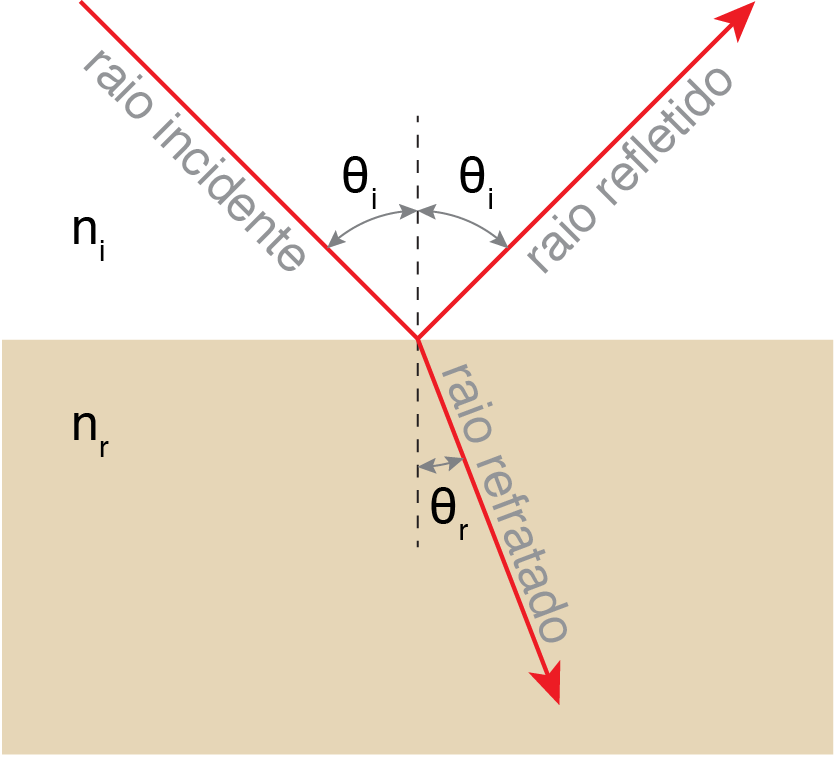
\includegraphics[width=0.4\textwidth]{1-snell}
%	\caption{. \label{fig:snell}} 
\end{figure}

\subsection{\sf Reflexão, refracção e polarização}

A eficiência com que um feixe luminoso é reflectido ou emitido numa fronteira entre dois meios de índices de refracção $n_1$ e $n_2$ depende, entre outros, do ângulo de incidência e da polarização da luz. A figura em baixo mostra como varia a reflectividade de uma superfície de vidro em função do ângulo de incidência, para polarizações horizontal e vertical (admitindo que o plano de incidência e reflexão é horizontal). Para um ângulo específico, designado ângulo de Brewster e dado por $\theta_B=\arctan(n_2/n_1)$, a componente horizontal da polarização não é reflectida, pelo que a luz reflectida fica com polarização vertical. Esta é uma forma de criar luz polarizada a partir de uma fonte não polarizada.

A figura ilustra também a geometria dos raios luminosos numa separação entre dois meios, no caso de incidência em ângulo de Brewster. Como se pode apreciar, nessa configuração o raio reflectido e o raio refractado fazem entre si um ângulo de 90$^\circ$.

\begin{figure}
	[!hb]  \centering 
	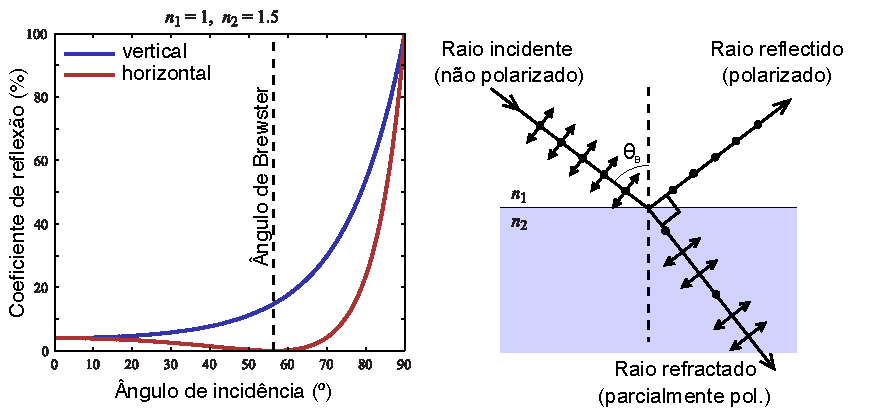
\includegraphics[width=0.8\textwidth]{2-brewster}
	\caption{Reflectividade vs. ângulo de incidência e direcção de polarização (esq.) e geometria para ângulo de Brewster (dir.). \label{fig:brewster}} 
\end{figure}



%%%%%%%%%%%%%%%%%%%%%%%%%%%%%%%%%%%%%%%%%%%%%%%%%%
%%%%%%%%%%%%%%%%%%%%%%%%%%%%%%%%%%%%%%%%%%%%%%%%%%
\section{\sf Construções geométricas em lentes delgadas (aproximação paraxial)}

Uma das principais aplicações da óptica geométrica consiste no estudo da formação de imagens: dado um objecto numa dada posição, como desenhar um sistema óptico que permita transferir uma imagem desse objecto para uma posição diferente? É um problema que tem aplicações desde o olho humano até ao desenho de lentes e fibras ópticas.

 Um \emph{objecto} iluminado uniformemente é considerado como uma fonte de raios, emitidos em todas as direcções. Podemos escolher um conjunto adequado de raios e traçar o seu percurso através do sistema, até encontrar o correspondente ponto na \emph{imagem}. Por convenção, desenha-se o sistema óptico em torno de um eixo, que coincide com o seu eixo geométrico, e os raios propagam-se da esquerda para a direita. 

\begin{figure}
	[!hb]  \centering 
	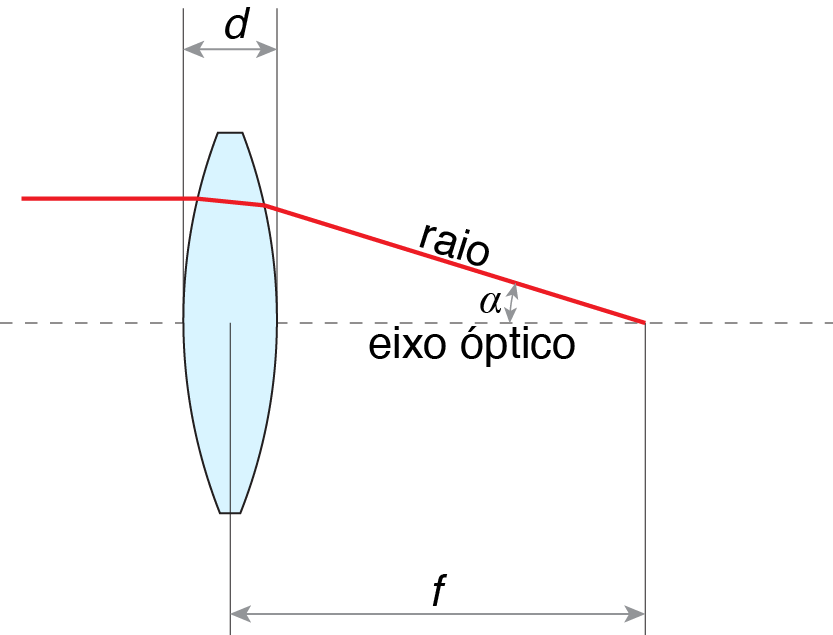
\includegraphics[width=0.4\textwidth]{2-definicoes}
 	\caption{\label{fig:fig2} Definições utilizadas: $f$ -- distância focal, $d<<f$ -- espessura da lente delgada, $\alpha$ -- ângulo entre o raio e o eixo óptico.} 
\end{figure}

\subsection{\sf Aproximações}
Utilizaremos as duas seguintes aproximações comuns, que facilitam grandemente os cálculos a efectuar:

\emph{Lentes delgadas} -- uma lente é considerada \emph{delgada} quando a sua espessura $d$ é desprezável face à sua distância focal $f$.

\emph{Aproximação paraxial} -- admitimos que todos os raios envolvidos são \emph{paraxiais}, isto é, (\emph{i}) situam-se próximo do eixo óptico e (\emph{ii}) o ângulo $\alpha$ que fazem com esse eixo permite utilizar as aproximações $\sin \alpha \approx \alpha$ e  $\tan \alpha \approx \alpha\,$, tipicamente válidas para $\alpha \leq \sim5^{\circ}$.


%%%%%%%%%%%%%%%%%%%%%%%%%%%%%%%%%%%%%%%%%%%%%%%%%%
\subsection{\sf Convenções}
A Figura \ref{fig:convencoes} ilustra os principais parâmetros envolvidos no traçado de raios através de uma lente simples.

\begin{itemize}
\item O objecto $AB$ fica (por definição) do lado esquerdo da lente, a uma distância $d_O>0$ desta; caso o objecto esteja do lado direito, temos $d_O<0$ (que é o caso do "objecto virtual" abordado mais à frente)
\item A imagem $A'B'$ está do lado direito da lente, a uma distância $d_I>0$ desta; ; caso a imagem esteja do lado esquerdo, temos $d_I<0$
\item $F_0$ é a distância focal do lado do objecto, $F_I$ é a distância focal do lado da imagem. No caso de uma lente fina, ambas são iguais a $f$, e marcam-se para auxiliar no traçado.
\end{itemize}


O raios ópticos que emergem de um dado objecto atravessam a lente e dão origem a uma imagem. As imagens dizem-se \emph{reais} quando os raios de luz passam de facto na posição da imagem, isto é, raios que saem do plano do objecto convergem no plano da imagem; e dizem-se \emph{virtuais} quando os raios não passam na imagem, mas esta é visível através da lente. As imagens reais podem ser projectadas num alvo, as virtuais não. Um bom exemplo é considerar a imagem de uma lâmpada brilhante: ao passar a mão pelo plano da imagem, se estar for real sente-se o calor, mas se for virtual parecerá apenas "flutuar" no espaço.

De seguida vamos analisar a formação de imagens para lentes convergentes ($f>0$) e divergentes ($f<0$) em função da posição relativa do objecto e do foco da lente, e derivar relações úteis para lentes delgadas.


%\begin{figure}	[!htb]  
%{\centering 
%	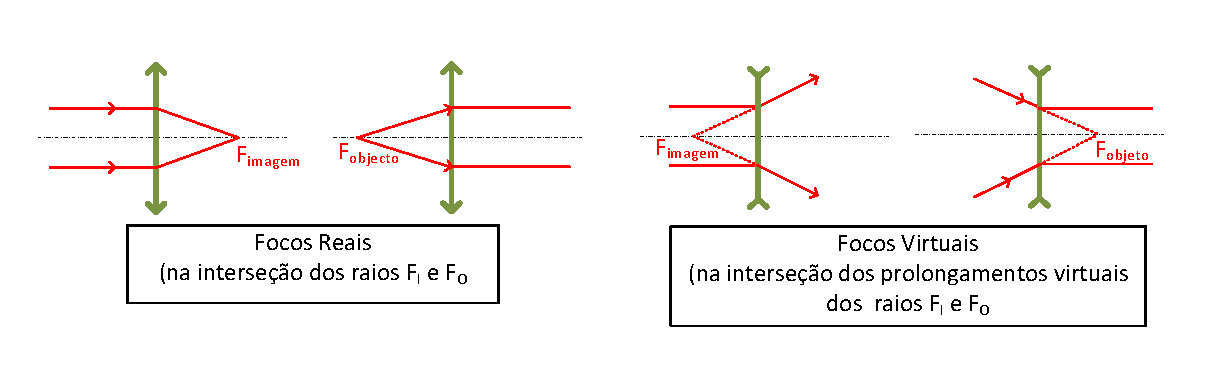
\includegraphics[width=\textwidth]{focoseImagem}
%	}
%	\caption{. \label{fig:focoseImagem}} 
%\end{figure}

\begin{figure}
	[!htb]  \centering 
	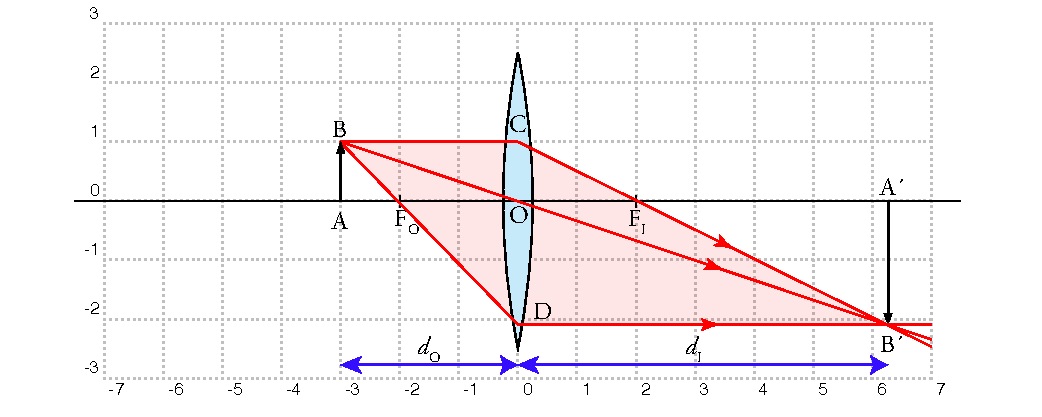
\includegraphics[width=1.0\textwidth]{3-convencoes}
	\caption{Convenções utilizadas para formação de imagens por lentes. \label{fig:convencoes}} 
\end{figure}

%\begin{figure}[t]
%\begin{pspicture}[showgrid=true](-7,-3)(7,3)
%\rput(0,0){\lens[focus=2,OA=-3,AB=1,XO=0,YO=0,nameF=F_0,nameFi=F_I,spotAi=0]}
%\rput{0}(0,1.4){C}
%\rput{0}(0,-2.4){D}
%\rput{0}(4,-0.4){2F$_0$}
%\rput{0}(-4,-0.4){2F$_0$}
%\end{pspicture}
%\caption{Convenções utilizadas para formação de imagens por lentes.} 
%\end{figure}

%%%%%%%%%%%%%%%%%%%%%%%%%%%%%%%%%%%%%%%%%%%%%%%%%%
\subsection{\sf Objecto e Imagem - Focos Conjugados}
Considere de novo a Fig. \ref{fig:convencoes}. Cada ponto do objecto em $d_O$ tem um único ponto correspondente na imagem em $d_I$. Isto implica que, caso colocássemos o objecto em $d_I$, a imagem seria formada em $d_O$. Chama-se a estas posições \emph{focos conjugados}.
Pela semelhança de triângulos temos as seguintes relações entre as dimensões do objecto e da imagem:

\begin{IEEEeqnarray}{rClrCl}
%\begin{array}{ccccc}
\Delta ABF_O \sim \Delta ODF_O  &\to & AB/A'B' = AF_O / F_O 0 &\to & AB/A'B' =  \frac{d_O-f}{ f} \label{eq:1} \\
\Delta ABO\sim \Delta A'B'O    &\to & AB/A'B' = AO / O A' &\to & AB/A'B' = d_O / d_I \label{eq:2} \\
\Delta COF_I \sim \Delta A'B'F_I  &\to & AB/A'B' = OF_I / F_I A' &\to & AB/A'B' =  \frac{f}{ d_I-f} \label{eq:3} 
\end{IEEEeqnarray}

Das expressões (\ref{eq:1}) e (\ref{eq:3}) obtemos a equação dos focos conjugados:
 
 \begin{equation}
	\label{eq:focosconjug}
    \fbox{
        $ \displaystyle
	\frac{1}{f} = \frac{1}{d_O} +\frac{1}{d_I} 
        $
    }
% \qquad \text{ equação dos focos conjugados}
\end{equation}

Por outro lado, sendo $AB$ e $A'B'$ respectivamente as dimensões lineares transversais do objecto e da imagem, usamos a igualdade (\ref{eq:2}) para definir a \emph{ampliação transversal} $A$ como:

 \begin{equation}
    \fbox{
        $ \displaystyle
A =  \frac{A'B'}{ AB} =\frac{d_I}{d_O}
$
}
\end{equation}
 
A imagem é \emph{direita} se $A<0$ e \emph{invertida} se $A>0$. Podemos usar estas duas equações para, dados $f$ e $d_O$, determinar as seguintes expressões para a posição da imagem $d_I$ e a respectiva ampliação $A$:
 
\begin{eqnarray}
A&=&\frac{1}{\frac{d_O}{f}-1}\\
d_I&=&d_OA
\end{eqnarray}

 
Como exemplo, temos no caso da Fig. \ref{fig:convencoes}: $d_O>f \to A> 0\,; d_I > 0$. A imagem resultante é \emph{real} e \emph{invertida}.

%%%%%%%%%%%%%%%%%%%%%%%%%%%%%%%%%%%%%%%%%%%%%%%%%%
\subsection{\sf Lente convergente ($f>0$) -- Imagem real}
Este caso verifica-se para $d_O>f$, a imagem é real é pode ser projectada. A imagem é maior ($A>1$) que o objecto se $d_O>2f$ ou menor ($A<1$) se $2f>d_O>0$. Um exemplo do primeiro caso é uma máquina fotográfica: a imagem é posicionada no sensor da câmara, e é (tipicamente) menor que o objecto fotografado. Verifica-se  \fbox{$0 < A \le 1$ } pois

\begin{equation}
\infty > d_O \ge 2 f \quad \to \quad f < d_I \le 2 f  \quad \to \quad 0<A\le 1
\end{equation}

Um exemplo do segundo caso é um projetor de cinema ou de imagem de computador: a imagem é posicionada num écran, e é maior que o objecto (película ou chip). Verifica-se  \fbox{$1 \le A < \infty$} pois

\begin{equation}
f < d_O \le 2 f  \quad \to  \quad  \infty > d_I \ge 2f \quad \to \quad \infty>A\ge 1
\end{equation}

%%%%%%%%%%%%%%%%%%%%%%%%%%%%%%%%%%%%%%%%%%%%%%%%%%
\subsection{\sf Lente convergente ($f>0$) -- Imagem virtual}

Este caso verifica-se quando $d_O<f$, por exemplo quando utilizamos uma lupa para ver objectos com um tamanho aumentado, e está esquematizada na Fig. \ref{fig:fig4}. Dependendo da posição $d_O$, verificam-se as seguintes relações

%\begin{figure}
%	[!htb]  \centering 
%	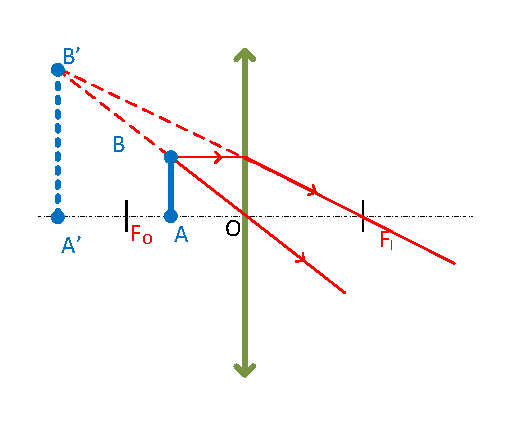
\includegraphics[width=0.8 \textwidth]{lupa}
%	\caption{. \label{fig:lupa}} 
%\end{figure}

\begin{IEEEeqnarray}{rCl}
0 < d_O \le \frac{f}{2} \qquad & 0 > d_I \ge -f \quad& -1 >A \ge -2\\
\frac{f}{2} \le d_O < f \qquad& -f\ge d_I >-\infty \quad& -2 > A > -\infty
\end{IEEEeqnarray}

Repare-se que resulta $d_I<0$ (a imagem está do mesmo lado que o objecto) e $A<0$ pelo que a imagem é (\emph{i}) virtual e (\emph{ii}) direita, para um observador colocado à direita da lente.

\begin{figure}
\begin{center}
\psscalebox{0.75}{
\begin{pspicture}[showgrid=true](-7,-3)(7,3)
\rput(0,0){\lens[lensType=CVG,focus=4.5,OA=-2.7,AB=1,XO=0,YO=0,nameF=F_O,nameFi=F_I,spotAi=0,drawing=true,rayColor=white]}
\psline[linecolor=red,linestyle=dashed](B')(F')
\psline[linecolor=red,linestyle=dashed](B')(B)
\psline[linecolor=red](B)(0,1)
\psline[linecolor=red](B)(2.7,-1)
\psline[linecolor=red](0,1)(F')
\psset{linecolor=red}
\Arrows[posStart=0,length=1](B)(0,1)
\Arrows[posStart=2,length=3](B)(0,0)
\Arrows[posStart=0,length=3](0,1)(F')
\rput(8,0){\psset{linecolor=black}\eye}
\end{pspicture}
}
\caption{Formação de imagem virtual com uma lente convergente. \label{fig:fig4}} 
\end{center}
\end{figure}

%%%%%%%%%%%%%%%%%%%%%%%%%%%%%%%%%%%%%%%%%%%%%%%%%%
\subsection{\sf Lente divergente ($f<0$)}


\begin{figure}
	[!htb]  \centering 
	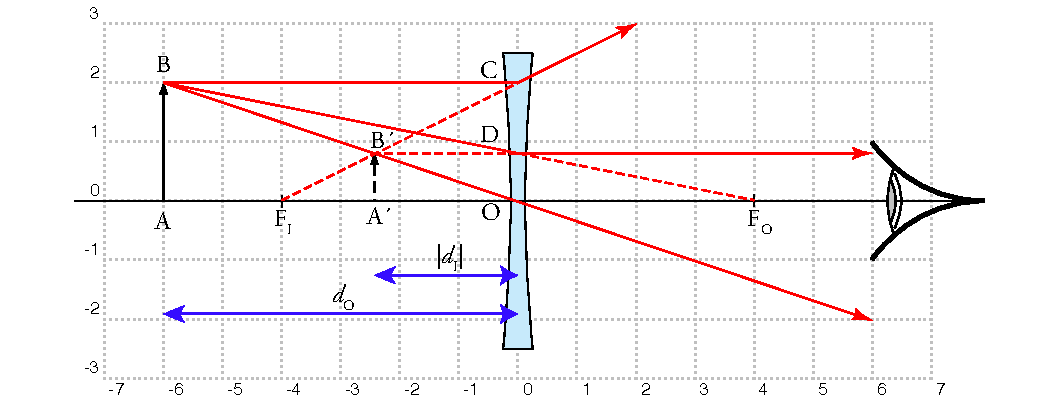
\includegraphics[width=0.7\textwidth]{5-DivVirt}
	\caption{Formação de imagem virtual com uma lente divergente. \label{fig:DivVirt}} 
\end{figure}

%\begin{figure}
%\begin{center}
%\psscalebox{0.75}{
%\begin{pspicture}[showgrid=true](-7,-3)(7,3)
%	\rput(0,0){\lens[lensType=DVG,focus=-2,spotAi=270,spotBi=90]} %nameF=F_1,
%	\rput(0,0){\lens[lensType=DVG,focus=-4,OA=-6,AB=2,XO=0,YO=0,nameF=F_O,nameFi=F_I,spotAi=0,drawing=true,rayColor=red]}
	%\uput[270](A){A}
	%\uput[270](F){F}
%	\uput[270](F'){$\mathrm{F'}$}
%	\rput(8,0){\psset{linecolor=black}\eye}
	%}
%\end{pspicture}
%}
%\caption{Formação de imagem virtual com uma lente divergente.}
%\end{center}
%\end{figure}

Considere-se a situação representada na Fig. \ref{fig:DivVirt}, que mostra uma lente divergente ($f<0$) e um objecto  $AB$ ($d_O>0$). Note-se que, no caso da lente divergente, os pontos $F_O$ e $F_I$ trocam de posição. Nesta configuração a imagem resultante $A'B'$ é sempre \emph{virtual}  e \emph{direita} com $d_I <0$ (imagem do mesmo lado do objeto), pois

\begin{equation*}
f<0; \quad d_O> 0 \quad \to  \quad A<0;  \quad  d_I <0  
\end{equation*}

Podemos verificar que a equação (\ref{eq:focosconjug}) se mantém válida neste caso, recorrendo à semelhança de triângulos:

\begin{IEEEeqnarray}{rClrCl}
%\begin{array}{ccccc}
\Delta ABO \sim  \Delta A'B'O  & \to & AB/A'B' = \frac{d_0}{d_I} & \to & -\infty < A < 0 \label{eq:diver1} \\
\Delta ABF_0\sim \Delta ODF_O   &\to & \frac{d_0 + |f|}{|f|} = AB/A'B' & \to & \frac{d_0 + |f|}{|f|} = \frac{d_0 }{d_I}  \label{eq:diver2} \\
\Delta F_I OC \sim \Delta F_I A'B'  &\to & \frac{|f|}{|f| - |d_I|} =AB/A'B'  &  \to &  \frac{|f|}{|f| - |d_I|} = \frac{d_0 }{|d_I|} 
\end{IEEEeqnarray}

Nestas expressões, que descrevem distâncias, foi necessário  utilizar os valores em módulo de $f$ e de $d_I$, que são ambos negativos. Fazendo agora as substituições $|f|\to -f$ e $|d_I|\to -d_I$ recupera-se a equação dos focos conjugados.


%%%%%%%%%%%%%%%%%%%%%%%%%%%%%%%%%%%%%%%%%%%%%%%%%%
\section{\sf Objetos virtuais ($d_O<0$)}

Em determinadas situações, podemos lidar com "objectos virtuais" -- isto é, os raios ópticos têm origem não num objecto sólido, mas num plano do espaço, e estamos interessados em estudar a sua propagação a partir desse plano e a formação da imagem correspondente. Um exemplo típico consiste em estudar a formação da imagem de uma imagem primária. Nestes casos, o objecto virtual é identificado a tracejado no diagrama de raios, como ilustrado nos exemplos em baixo.

%%%%%%%%%%%%%%%%%%%%%%%%%%%%%%%%%%%%%%%%%%%%%%%%%%
\subsection{\sf Lente convergente}
A Fig. \ref{fig:ConvVirt} representa um objecto virtual ($d_O<0$, à direita da lente) e a correspondente imagem. A imagem resultante é real ($d_I>0$, também à direita) e direita ($A<0$), verificando-se

\begin{IEEEeqnarray}{rCl}
 d_O < 0 ; \quad &&  f > 0 \quad \to \quad A<0  \nonumber\\
\frac{d_I}{-|d_O|}  & =&  \frac{f}{-|d_O| -f}     \nonumber
\end{IEEEeqnarray}



\begin{figure}
	[!htb]  \centering 
	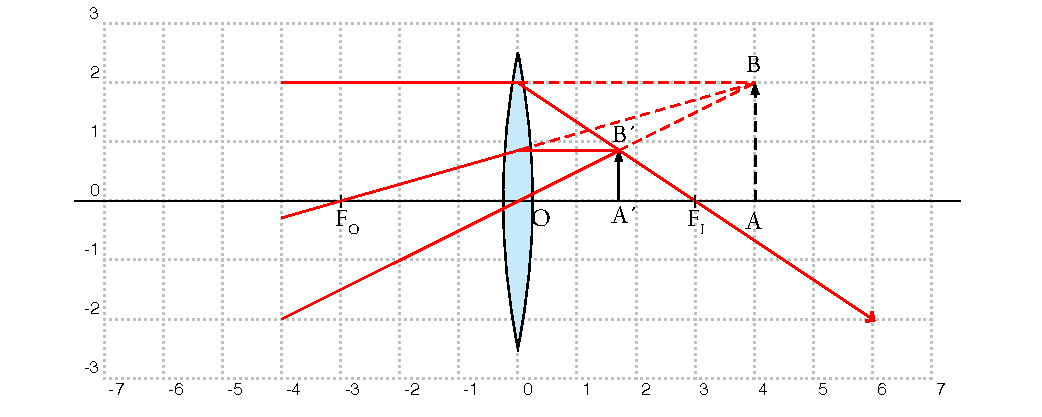
\includegraphics[width=0.7\textwidth]{6-ConvVirt}
	\caption{Lente convergente com objecto virtual e imagem real. \label{fig:ConvVirt}} 
\end{figure}


%\begin{minipage}[c]{0.6\textwidth}
%\begin{figure}
%	[!htb]  \centering 
%	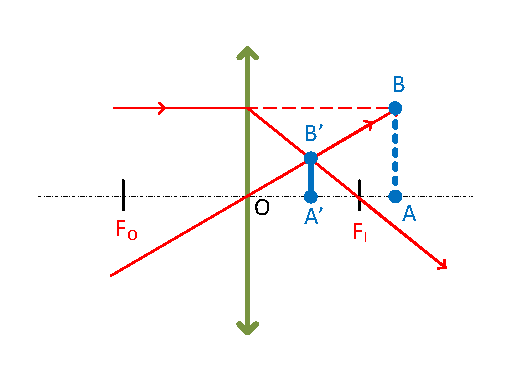
\includegraphics[width=\textwidth]{convergVirt}
%	\caption{. \label{fig:lupa}} 
%\end{figure}
%\end{minipage}
%\begin{minipage}[c]{0.4\textwidth}
% \end{minipage}

%Do objeto virtual obteve-se uma imagem \textbf{real} e \textbf{direita}.

%%%%%%%%%%%%%%%%%%%%%%%%%%%%%%%%%%%%%%%%%%%%%%%%%%
\subsection{\sf Lente divergente -- Imagem virtual}

\begin{figure}
	[!htb]  \centering 
	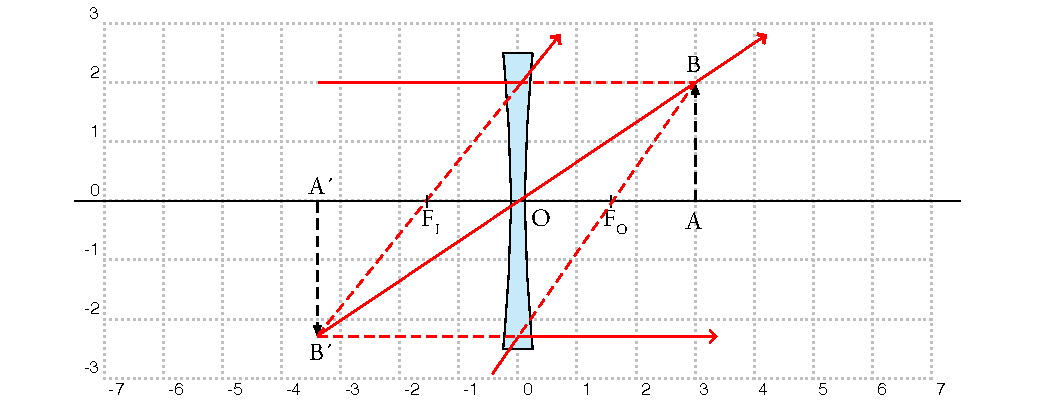
\includegraphics[width=0.7\textwidth]{7-DivVirtVirt}
	\caption{Lente divergente com objecto virtual e imagem virtual. \label{fig:DivVirtVirt}} 
\end{figure}

A Fig. \ref{fig:DivVirtVirt} representa um objecto virtual ($d_O<0$, à direita da lente) para uma lente divergente ($f<0$) e a correspondente imagem. Na situação da figura, o objecto está à direita do foco $F_O$: $|d_O|>|f|$. Verifica-se assim:

\begin{IEEEeqnarray}{rCl}
 d_O < 0 & &  f < 0   \nonumber\\
\frac{d_I}{|d_O|}  & =&  \frac{|f|}{|d_O| -|f|}     \nonumber
\end{IEEEeqnarray}

A imagem resultante é também virtual $d_I<0$, à esquerda da lente) e invertida ($A>0$), verificando-se as seguintes relações em função da distância:
\begin{equation}
|d_O|  =  \left\{
\begin{array}{rl}
|d_O|   = |f|:  &   |d_I| \to \infty, \quad A \to \infty ,\\
|f| < |d_O|   < 2|f|:  &   |d_I|  > |d_O| , \quad A  >1  ,\\
|d_O|   = 2|f|:  &   |d_I| = |d_O|, \quad A =1  ,\\
|d_O|  > 2|f|:   & |d_I|  <|d_O| , \quad 0 < A  <1  .
\end{array}  \right.
%f<0 \quad \to   d_O> 0 ; \quad  d_I <0  
\end{equation}

%%%%%%%%%%%%%%%%%%%%%%%%%%%%%%%%%%%%%%%%%%%%%%%%%%
\subsection{\sf Lente divergente - Imagem real}

A Fig. \ref{fig:DivVirtReal} representa um objecto virtual ($d_O<0$, à direita da lente) para uma lente divergente ($f<0$) e a correspondente imagem. Na situação da figura, o objecto está à esquerda do foco $F_O$: $|d_O|<|f|$. Verifica-se assim:

\begin{figure}
	[!htb]  \centering 
	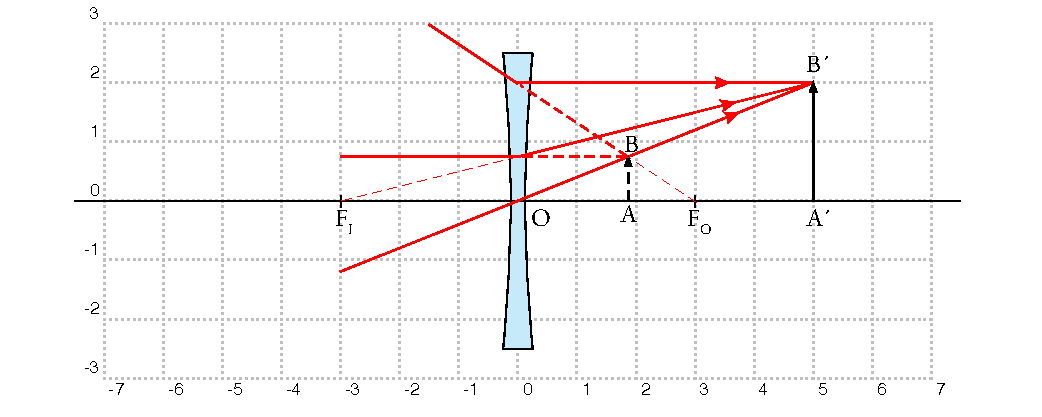
\includegraphics[width=0.7\textwidth]{8-DivVirtReal}
	\caption{Lente divergente com objecto virtual e imagem real. \label{fig:DivVirtReal}} 
\end{figure}

\begin{IEEEeqnarray}{rCl}
 d_O < 0 & &  f < 0   \nonumber\\
\frac{d_I}{|d_O|}  & =&  \frac{|f|}{|f|-|d_O|} \quad \to \quad A=\frac{d_I}{d_O} =\frac{f}{d_O-f}<0     \nonumber
\end{IEEEeqnarray}

%\begin{IEEEeqnarray}{rCl}
%\textrm{Se } d_O < 0 ; \quad  |d_O| <  |f|; \quad  |d_O| <  x|f| ; \quad (x < 1) & \to &    d_I >0; \quad A > 1 \nonumber
%\end{IEEEeqnarray}

A imagem resultante é agora real ($d_I>0$, à direita da lente) e direita ($A<0$), verificando-se as seguintes relações em função da distância:
\begin{equation}
|d_O|  =  \left\{
\begin{array}{rl}
|d_O|   \to |f|:  &   |d_I| \to \infty, \quad A \to -\infty ,\\
|d_O|   = |f|/2:  &   |d_I| = f, \quad A =-2  ,\\
|d_O|  =0:  & |d_I|  =0 , \quad A=-1.
\end{array}  \right.
%f<0 \quad \to   d_O> 0 ; \quad  d_I <0  
\end{equation}


%\begin{figure}	[!htb]  \centering 
%	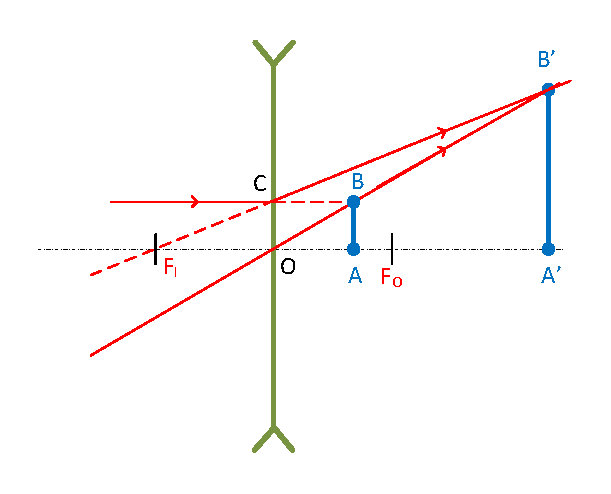
\includegraphics[width=\textwidth]{divergReal}
%	\caption{. \label{fig:lupa}} 
%\end{figure}

%%%%%%%%%%%%%%%%%%%%%%%%%%%%%%%%%%%%%%%%%%%%%%%%%%
%%%%%%%%%%%%%%%%%%%%%%%%%%%%%%%%%%%%%%%%%%%%%%%%%%
\section{\sf Associação de lentes delgadas}

Para duas lentes delgadas de distâncias focais $f_1$ e $f_2$ afastadas de $D$ (para $D \ll f_1,f_2$) pode calcular-se a distância focal equivalente do conjunto através de: 

 \begin{equation}
	\label{eq:assoclentes}
    \fbox{
        $ \displaystyle
	\frac{1}{f_{equiv}} = \frac{1}{f_1} + \frac{1}{f_2} - \frac{D}{f_1 \,f_2} 
        $
    }
\end{equation}

A dificuldade
%quando se usa o método direto quer dos focos conjugados, para 
na determinação da distância focal equivalente ${f_{equiv}}$ é a medição das distâncias $d_O$ e $d_I$ 
(que são diferentes das distância do objecto e da imagem às superfícies das lentes ou aos seus planos médios).

Uma abordagem preferível consiste em usar a equação (\ref{eq:focosconjug}) separadamente para cada uma das lentes, e considerar que a \emph{primeira imagem} (real ou virtual) irá constituir-se como o \emph{objecto} para a segunda lente. Vamos aplicar este método para várias combinações.

%%%%%%%%%%%%%%%%%%%%%%%%%%%%%%%%%%%%%%%%%%%%%%%%%%
\subsection{\sf Duas lentes convergentes afastadas de $D$}
A figura \ref{fig:DuplaConvConv1} representa duas lentes, $L_1$ e $L_2$, de distâncias focais $f_1$ e $f_2$ respectivamente, separadas de uma distância $D$. O objecto (real) $AB$ situa-se à esquerda de $L_1$, e tem uma imagem $A'B'$ por intermédio de $L_1$. Esta imagem constitui-se como objecto virtual para $L_2$, resultando no final a imagem $A''B''$.

\begin{figure}	[!htb]  \centering 
	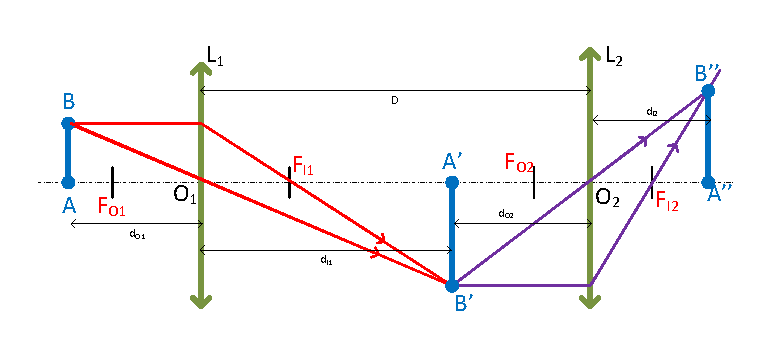
\includegraphics[width=0.9\textwidth]{9-DuplaConvConv1}
	\caption{Sistema de duas lentes convergentes. \label{fig:DuplaConvConv1}} 
\end{figure}

%\begin{pspicture*}(-7.5,-3)(7.5,3)
%	\rput(0,0){\lens[lensScale=0.6,XO=-4,AB=1,nameF=F_{O1},nameA=A_1,nameB=B_1,
  %		nameFi=F_{I1},nameAi={ },nameBi={},nameO=O_1,focus=1,OA=-2,lensGlass=true, lensWidth=0.5]}
	%\pspolygon[style=rayuresJaunes,linestyle=none](B)(I)(B')(I')(B)
%	\Transform
%	\rput(0,0){\lens[lensScale=0.8,XO=2,focus=2,nameA=A'_1,spotA=90,nameB=B'_1,spotB=270,
 % 		nameO=O_2,nameAi=A'',spotAi=270,nameBi=B'',spotBi=90,nameF=F_{O2},nameFi=F_{I2},
 % 		lensTwo=true,lensGlass=true,lensWidth=0.5]}
	%\pspolygon[style=rayuresJaunes,linestyle=none](B)(I)(B')(I')(B)
%\end{pspicture*}

Apliquemos as equações de lentes individuais para cada caso:

\begin{equation}
|d_O|  =  \left\{
\begin{array}{llll}
 \frac{1}{d_{O_1}} +  \frac{1}{d_{I_1}}   = \frac{1}{f_1}  & d_{O_1} = AO_1 & d_{I_1} = O_1A' & f_1 = O_1 F_{O_1} = O_1\,F_{I_1} \\
 \frac{1}{d_{O_2}} +  \frac{1}{d_{I_2}}   = \frac{1}{f_2}  & d_{O_2} = A'O_2 & d_{I_2} = O_2\,A'' & f_2 =  F_{O_2}\,O_2\, = O_2\,F_{I_2} \\
O_1\,O_2 = D = d_{I_1} + d_{O_2}
\end{array}  \right.
\label{eq:assoclentes_2}
\end{equation}

Esta é a montagem mais simples de um \textbf{telescópio}, a partir do qual se podem obter grandes ampliações.
Estas três expressões permitem calcular o valor de uma das incógnitas, conhecidos os valores das outras; por exemplo, podemos determinar $f_2$, conhecidos os valores de $f_1$, $d_{O_1}$, $d_{I_2}$ e $D$.

As mesmas expressões aplicam-se para o caso de uma imagem obtida por uma lente $L_1$ que passa a ser um “objecto” virtual para $L_2$, isto é, em que $d_{O2}<0$, situação ilustrada na Fig. \ref{fig:DuplaConvConv2}.

\begin{figure}	[!htb]  \centering 
	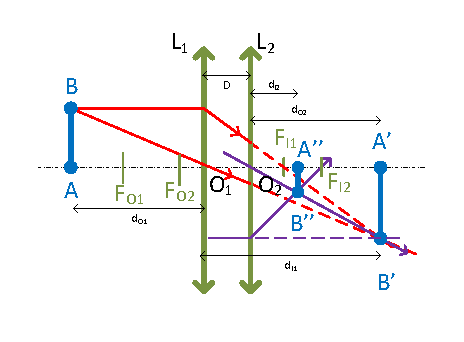
\includegraphics[width=0.9\textwidth]{10-DuplaConvConv2}
	\caption{Duas lentes convergentes, com objecto intermédio virtual. \label{fig:DuplaConvConv2}} 
\end{figure}

%%%%%%%%%%%%%%%%%%%%%%%%%%%%%%%%%%%%%%%%%%%%%%%%%%
\subsection{\sf Lentes convergente e divergente afastadas de $D$}
O outro sistema de lente dupla de interesse é o caso em que temos uma lente convergente e uma divergente separadas de $D$, ilustrado na Fig. \ref{fig:DuplaConvDiv1}, em que $L_1$ é convergente e $L_2$ é divergente. A lente $L_1$ produz uma imagem intermédia $A'B'$ real e invertida, que é o objecto (real) de $L_2$. Uma vez que a segunda lente é divergente, a sua imagem $A''B''$ (a imagem final) é sempre virtual e invertida.

\begin{figure}	[!htb]  \centering 
	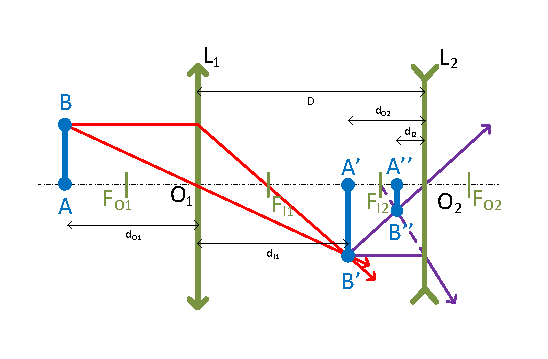
\includegraphics[width=0.9\textwidth]{11-DuplaConvDiv1}
	\caption{Sistema de lente convergente e divergente. A imagem final é sempre virtual e invertida. \label{fig:DuplaConvDiv1}} 
\end{figure}

A figura \ref{fig:DuplaConvDiv2} ilustra a situação em que $A'B'$ está numa posição à direita de $L_2$: é uma imagem real (de $L_1$) mas um objecto virtual (de $L_2$), já que $d_{O2}<0$. A imagem $A''B''$ resultante é real e invertida.

\begin{figure}	[!htb] 
\begin{center}
	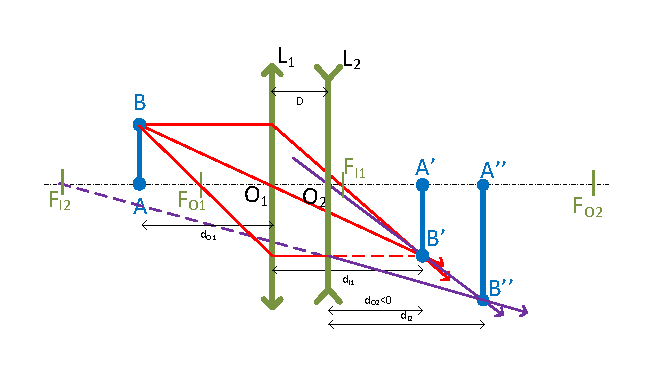
\includegraphics[width=0.9\textwidth]{12-DuplaConvDiv2}
	\caption{Sistema de lente convergente e divergente com objecto (intermédio) virtual. A imagem final é real e invertida. \label{fig:DuplaConvDiv2}} 
\end{center}
\end{figure}

\begin{figure}	[!htb]  
\begin{center}
	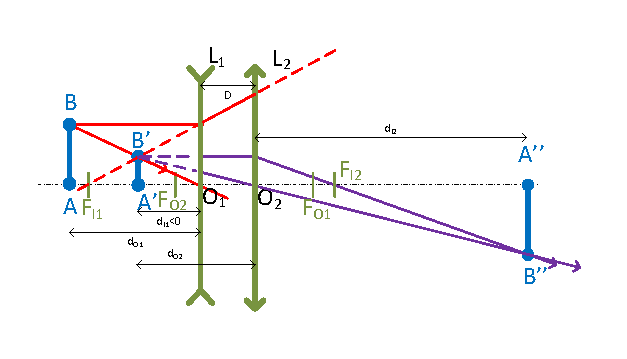
\includegraphics[width=0.9\textwidth]{13-DuplaConvDiv3}
\end{center}
	\caption{Sistema de lente convergente e divergente.  \label{fig:DuplaConvDiv3}} 
\end{figure}


Se $L_1$ e $L_2$ permutarem (Fig. \ref{fig:DuplaConvDiv3}), obtém-se também uma imagem real  $A''\,B''$ desde que a distância $d_{O1}=A\,O_1$ seja idêntica.
Em qualquer destas situações, pode sempre calcular-se $f_2 < 0$ usando o conjunto das três equações (\ref{eq:assoclentes_2}).
\clearpage


%%%%%%%%%%%%%%%%%%%%%%%%%%%%%%%%%%%%%%%%%%%%%%%%%%
%\section{Microscópio}

%\begin{LTXexample}
%\begin{pspicture}(-7.5,-5.5)(7.5,3)
%\rput(0,0){\lens[focus=1.5,OA=-2,AB=0.5,XO=-5,lensGlass=true,lensWidth=0.4,
%   yBottom=-4,yTop=4,drawing=false,lensScale=0.4,nameF=F_1,nameFi=F'_1]
%  \psline[linewidth=1pt](xLeft)(xRight)}
%\pnode(! XO 1){UPlens1} \pnode(! XO -1){DOWNlens1}
%\Transform
%\rput(0,0){\lens[focus=2,XO=3,lensGlass=true,lensWidth=0.4,yBottom=-4,yTop=4,drawing=false,
%        nameF=F_2,nameFi=F'_2,spotF=90,spotFi=90]}
%\psline{->}(A1)(B1)\psline{->}(A'1)(B'1)\uput[270](A1){A}\uput[90](B1){B}
%\uput[270](B'1){$\mathrm{B_1}$}\uput{0.7}[90](A'1){$\mathrm{A_1}$}
%{\psset{linecolor=red}
% \rayInterLens(I11)(B'1){3}{Inter1L2}\rayInterLens(B1)(O1){3}{Inter2L2}
% \rayInterLens(UPlens1)(B'1){3}{Inter3L2}\rayInterLens(DOWNlens1)(B'1){3}{Inter4L2}
% \psline(B1)(I11)(B'1)(Inter1L2)\psline(B1)(Inter2L2)\psline(B1)(UPlens1)(Inter3L2)
% \psline(B1)(DOWNlens1)(Inter4L2)
% \psset{length=5}
% \Parallel(B'1)(O)(Inter3L2){B1inftyRigth}\Parallel(B'1)(O)(Inter4L2){B2inftyRigth}
% \Parallel(B'1)(O)(Inter2L2){B3inftyRigth}\Parallel(B'1)(O)(Inter1L2){B3inftyRigth}
% {\psset{length=-5,linestyle=dashed}
%  \Parallel(B'1)(O)(Inter3L2){B1inftyLeft}\Parallel(B'1)(O)(Inter4L2){B2inftyLeft}
%  \Parallel(B'1)(O)(Inter2L2){B3inftyLeft}\Parallel(B'1)(O)(Inter1L2){B3inftyLeft}
%  \pcline[nodesep=6](B'1)(O)}
% \pspolygon[style=rayuresJaunes,linestyle=none](B1)(UPlens1)(Inter3L2)%
% 	(B1inftyRigth)(B2inftyRigth)(Inter4L2)(DOWNlens1)
% \psline(B1)(UPlens1)(Inter3L2)(B1inftyRigth)\psline(B2inftyRigth)(Inter4L2)(DOWNlens1)(B1)}
%\rput(7,0){\eye}
%\end{pspicture}%



%%%%%%%%%%%%%%%%%%%%%%%%%%%%%%%%%%%%%%%%%%%%%%%%%%

\section{\sf Protocolo Experimental}

%\subsection{\sf Questões a responder ANTES da sessão de Laboratório:}
%\begin{enumerate}
%\item Descreva por palavras suas quais os objectivos do Trabalho que irá realizar na sessão de Laboratório (uma folha A4). Indique as expressões que irá utilizar para obter as grandezas experimentais, bem como as expressões para calcular as incertezas. Inclua esta parte também no Relatório. Este irá constituir o ÚNICO meio de consulta na Prova Individual.
	
% \item Utilizando uns óculos graduados (se não usar, peça a um colega), obtenha e registe a sua graduação. Calcule a distância focal, $f=1/$Dioptrias (para miopia são lentes divergentes, para hipermetropia são convergentes. Ignore  a correção do astigmatismo).
%\item Classifique as imagens visualizadas através das lentes, i.e: Reais/Virtuais, Direitas/Invertidas, Ampliadas/Reduzidas, Posição da Imagem relativa aos objetos.
%\item Para uma lente de $-2.5$ Dioptrias calcule a posicão da imagem para um objeto a 40 cm da lente. A que distância está do objeto?
%\item Para uma lente convergente (óculos ou uma lupa) em que condições obtém uma imagem virtual: a) direita; b) invertida?
%\end{enumerate}

\subsection{\sf Material utilizado}
\begin{itemize}
\item caixa de óptica equipada com calha graduada
\item lentes convergentes e divergente
\item semi-cilindro de vidro acrílico
\item diafragmas
\item polaroides
\item suportes
\item fonte luminosa com lâmpada de incandescência linear
\end{itemize}


%%%%%%%%%%%%%%%%%%%%%%%%%%%%%%%%%%%%%%%%%%%%%%%%%%

\subsection{\sf Procedimento Experimental}

\subsubsection{\sf  Índice de refracção dum vidro acrílico }

\begin{enumerate}
\item Utilizando a  fonte  luminosa  obtenha  um  feixe  de  luz  branca  de  raios  paralelos. Que tipo de lente necessita?
\item Com os diafragmas obtenha um feixe de luz estreito ($\approx$ 1 mm), alinhado com o eixo do Transferidor.
\item Faça  incidir  luz  branca  na  superfície  plana  do  semi-cilindro  de  vidro  acrílico.  Observe  e obtenha os ângulos de 
reflexão e a transmissão para vários ângulos do feixe incidente, à 
esquerda e à direita.  Faça  medições  pelo  menos  para  nove  valores  diferentes  do 
ângulo de incidência.
\item  Determine \emph{a partir do gráfico}, por ajuste, o índice de refracção do vidro acrílico.  
\item Repita  as  medidas  e  a  análise  dos  resultados  fazendo  agora  a  incidência  na  superfície cilíndrica. 
\item  Compare o índice de refracção do vidro acrílico a partir da incidência nas duas faces. 
\item Estime também o valor do índice de refracção a partir do ângulo limite de reflexão total. 
\item  Compare a precisão dos diferentes valores obtidos de $n_{vidro}$. 
\end{enumerate}

%%%%%%%%%%%%%%%%%%%%%%%%%%%%%%%%%%%%%%%%%%%%%%%%%%
\subsubsection{\sf Polarização da luz. Ângulo de Brewster}
Observe o efeito de interposição de dois polaroides paralelos ou cruzados no percurso de um feixe luminoso. 
Usando a mesma montagem do ponto anterior, polarize o feixe  paralelamente ao plano
de incidência, orientando o eixo $0^\circ-180^\circ$ do polarizador na vertical. Para valores do ângulo de incidência próximos 
do  ângulo  de  Brewster  (que  pode  calcular  a  partir  do  índice de refracção) obtenha   o  intervalo 
angular em que se extingue praticamente o feixe reflectido. 

%%%%%%%%%%%%%%%%%%%%%%%%%%%%%%%%%%%%%%%%%%%%%%%%%%
\subsubsection{\sf   Distância focal de uma lente convergente ( $f  \approx$ 75 mm) }
 
\begin{enumerate}
\item Obtenha  um  feixe  de  luz  branca  de  raios  paralelos, usando a lente colimadora.
Determine  a  distância  focal (d.f.)  da  lente pelo método directo.  Repita  a  experiência  duas  vezes,  colocando  a  lente 
noutra posição relativamente à lente de raios paralelos. 
\item Coloque o \emph{objeto} com mira no suporte da calha, iluminando-o directamente com a fonte luminosa. Coloque a mesma lente convergente a uma distância 150 mm $< d_O <$ 75 mm do objeto.

\item Com o écran plano procure a posição correcta para obter uma \emph{imagem} focada.
Utilizando a equação dos focos conjugados, calcule de novo a d.f. da lente. 
\item Na folha quadriculada em anexo desenhe um diagrama com o eixo óptico, o objecto e a lente convergente. Utilizando as aproximações paraxial e das lentes delgadas desenhe a construção geométrica e obtenha a posição da imagem e a respectiva ampliação.

\item Medindo agora a imagem determine a ampliação linear. Compare-a com a que podia  calcular pelas distância $d_O$  e $d_I$. 
\item Repita a experiência duas vezes, colocando a lente noutras posições relativamente ao objecto.  
\item Compare o valor da distância focal com o obtido em a) e estime a precisão envolvida em 
cada um dos métodos que utilizou. 
\end{enumerate}

%%%%%%%%%%%%%%%%%%%%%%%%%%%%%%%%%%%%%%%%%%%%%%%%%%
\subsubsection{\sf   Distância focal de uma lente divergente ( $f  \approx$ --150 mm) }
\begin{enumerate}
\item Associe  no  mesmo  suporte  a  lente  divergente  com  uma  convergente ($f  \approx$ 75 mm) de  forma a  que  o 
conjunto se comporte como um sistema convergente (com $D\approx 0$).
\item Repita a montagem com objecto e a sua imagem real. 
%\item Conhecidas  a  distância  focal  da  lente  convergente  e  a  distância  entre  lentes $D$, calcule  a distância focal da lente divergente a partir de $d_O$  e $d_I$. 
%\item Repita a experiência (pelo menos uma vez), colocando o conjunto das lentes noutra posição relativamente ao objeto. 


\end{enumerate}
	
\newpage
\def\width{18}
\def\hauteur{25}
\begin{tikzpicture}[x=1cm, y=1cm, semitransparent]
\draw[step=1mm, line width=0.1mm, black!30!white] (0,0) grid (\width,\hauteur);
\draw[step=5mm, line width=0.2mm, black!40!white] (0,0) grid (\width,\hauteur);
\draw[step=5cm, line width=0.5mm, black!50!white] (0,0) grid (\width,\hauteur);
\draw[step=1cm, line width=0.3mm, black!90!white] (0,0) grid (\width,\hauteur);
\end{tikzpicture}


\end{document} 